\section{Odd-Even Transposition Sort}

\subsection{Introduction}
\textbf{History:} Developed in 1972 by N. Habermann for parallel processor arrays, OETS gained prominence through Kenneth Batcher's work on sorting networks. Its design enables efficient execution on architectures with local interconnections, predating modern GPU-based sorting techniques.

\begin{figure}[H]
\centering
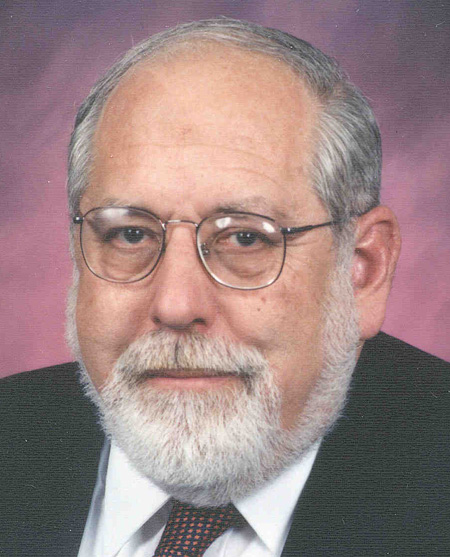
\includegraphics[scale = 0.5]{img/kennethEBatcher.jpg}
\caption{Kenneth Batcher (1935-2019)}
\label{fig:batcher}
\end{figure}

\textbf{Definition:} Odd-Even Transposition Sort (OETS) is a parallel sorting algorithm derived from Bubble Sort, using alternating comparison phases to enable efficient concurrent execution. It operates in $O(n^2)$ time sequentially but achieves $O(n)$ time with $n$ processors in parallel implementations. The algorithm's simplicity and parallelizability make it valuable for multi-core systems and educational demonstrations.

\subsection{Algorithm and Implementation}
\begin{itemize}
    \item \textbf{Array:} The algorithm operates on a 1D array, comparing and swapping adjacent elements in-place.
    \item \textbf{Parallel Processors:} Each processor holds one element and communicates with immediate neighbors during odd/even phases.
\end{itemize}

\begin{algorithm}
    \caption{Odd-Even Transposition Sort}
    \begin{algorithmic}[1]
        \State \textbf{Input:} Array $A$ of size $n$
        \State \textbf{Output:} Sorted array $A$
        \Function{OddEvenSort}{$A$, $n$}
            \State $isSorted \gets \text{False}$
            \While{$\neg isSorted$}
                \State $isSorted \gets \text{True}$
                \For{$i \gets 1$ to $n-1$ \textbf{step} 2}
                    \If{$A[i] > A[i+1]$}
                        \State \Call{swap}{$A[i], A[i+1]$}
                        \State $isSorted \gets \text{False}$
                    \EndIf
                \EndFor
                \For{$i \gets 0$ to $n-1$ \textbf{step} 2}
                    \If{$A[i] > A[i+1]$}
                        \State \Call{swap}{$A[i], A[i+1]$}
                        \State $isSorted \gets \text{False}$
                    \EndIf
                \EndFor
            \EndWhile
        \EndFunction
    \end{algorithmic}
\end{algorithm}

Below is the implementation in C++:

\lstinputlisting[language=C++, caption=Odd-Even Transposition Sort in C++]{code/oddEvenSort.cpp}

\subsection{Evaluation}
\subsubsection{Building the Even-Odd Transposition Sort Array}
\textbf{Operation:} Create and set up the array for sorting the input elements. \\
\textbf{Complexity:} $O(n)$ \\
\textbf{Explanation:} The initial setup involves creating an array of size $n$ (where $n$ is the number of elements to be sorted). This is a straightforward operation that requires linear time to allocate memory for the array.

\subsubsection{Filling the Even-Odd Transposition Sort Array}
\textbf{Operation:} Distribute elements from the input array into the sorting process. \\
\textbf{Complexity:} $O(n)$ \\
\textbf{Explanation:} The algorithm traverses through the input array to perform comparisons and swaps. Each element is compared with its adjacent elements in both the even and odd phases. This requires a linear traversal of the array, leading to a time complexity of $O(n)$ for each phase.

\subsubsection{Even Phase of the Sort}
\textbf{Operation:} Compare and swap adjacent elements at even indices. \\
\textbf{Complexity:} $O(n)$ \\
\textbf{Explanation:} In the even phase, the algorithm iterates through the array, comparing pairs of elements at even indices. Each comparison and potential swap takes constant time, resulting in a linear time complexity for this phase.

\subsubsection{Odd Phase of the Sort}
\textbf{Operation:} Compare and swap adjacent elements at odd indices. \\
\textbf{Complexity:} $O(n)$ \\
\textbf{Explanation:} Similar to the even phase, the odd phase involves iterating through the array and comparing pairs of elements at odd indices. This also results in a linear time complexity.

\subsubsection{Overall Sorting Process}
\textbf{Operation:} Repeat the even and odd phases until the array is sorted. \\
\textbf{Complexity:} $O(n^2)$ (in the average and worst cases) \\
\textbf{Explanation:} The even and odd phases are repeated until no swaps are made. In the worst case, the algorithm may need to perform $n$ passes through the array, leading to a quadratic time complexity of $O(n^2)$.

\subsubsection{Space Complexity}
\textbf{Operation:} Memory usage during sorting. \\
\textbf{Complexity:} $O(1)$ \\
\textbf{Explanation:} The Even-Odd Transposition Sort is an in-place sorting algorithm, meaning it does not require additional storage proportional to the input size. Only a constant amount of extra space is used for variables (like loop counters and flags).

\subsection{Applications}
While the even-odd transposition sort is not commonly used in practical applications due to its inefficiency compared to other sorting algorithms, it has some niche applications, particularly in educational contexts and parallel computing:
\begin{itemize}
    \item \textbf{Educational Purposes:} The algorithm is often used in computer science courses to teach sorting algorithms and the concept of parallel processing. It helps students understand how sorting can be performed in a distributed manner.
    \item \textbf{Parallel Computing:} In environments where multiple processors are available, the even-odd transposition sort can be implemented to take advantage of parallelism. Each phase (even and odd) can be executed simultaneously on different processors, making it suitable for parallel architectures.
    \item \textbf{Sorting Networks:} The even-odd transposition sort is related to sorting networks, which are used in hardware implementations of sorting algorithms. These networks can be used in applications where sorting needs to be done quickly and efficiently in hardware.
\end{itemize}

\subsection{Problems}

\subsubsection{Sort Colors}
\href{https://leetcode.com/problems/sort-colors/description/}{LeetCode}

\textbf{Description:} Given an array with $n$ objects colored red, white, or blue, sort them in-place so that objects of the same color are adjacent, with the colors in the order red, white, and blue.

\textbf{Detailed Instructions:}
\begin{enumerate}
    \item Initialize Pointers: Set three pointers: low, mid, and high. Initialize low and mid to the start of the array and high to the end.
    \item Iterate Through the Array:
    \begin{itemize}
        \item While mid is less than or equal to high:
        \item If array[mid] is 0, swap it with array[low], increment both low and mid.
        \item If array[mid] is 1, just increment mid.
        \item If array[mid] is 2, swap it with array[high] and decrement high.
    \end{itemize}
    \item Complete the Sorting: Continue until mid exceeds high.
    \item Return the Sorted Array.
\end{enumerate}

\subsubsection{Sorting: Bubble Sort}
\href{https://www.hackerrank.com/challenges/30-sorting/problem}{HackerRank}

\textbf{Description:} Given an array of integers, perform a bubble sort and count the number of swaps that are made. Print the number of swaps and the first and last elements of the sorted array.

\textbf{Detailed Instructions:}
\begin{enumerate}
    \item Initialize Variables: Create a variable to count swaps and initialize it to zero.
    \item Use a nested loop: the outer loop runs from 0 to $n-1$, and the inner loop runs from 0 to $n-i-1$.
    \item Compare adjacent elements and swap them if they are in the wrong order.
    \item Increment the swap counter each time a swap is made.
    \item Output the Results: After sorting, print the total number of swaps, the first element, and the last element of the sorted array.
    \item Return the Output.
\end{enumerate}

\subsubsection{A. Sort the Array}
\href{https://codeforces.com/problemset/problem/1360/A}{Codeforces}

\textbf{Description:} You are given an array of integers. You need to determine if it is possible to sort the array by performing a certain number of operations. Each operation consists of choosing two indices and swapping the elements at those indices.

\textbf{Detailed Instructions:}
\begin{enumerate}
    \item Check for Sortedness: If the array is already sorted, output "YES".
    \item Count Odd and Even Elements: If the array is not sorted, check if the odd and even indexed elements can be sorted independently.
    \item Sort the Array: Create a copy of the array and sort it.
    \item Compare: Check if the sorted array can be obtained by sorting the original array's odd and even indexed elements separately.
    \item Output the Result: If it is possible to sort the array, print "YES"; otherwise, print "NO".
\end{enumerate}

\subsubsection{Merge Intervals}
\href{https://leetcode.com/problems/merge-intervals/}{LeetCode}

\textbf{Description:} Given a collection of intervals, merge all overlapping intervals.

\textbf{Detailed Instructions:}
\begin{enumerate}
    \item Sort the Intervals: First, sort the intervals based on the starting times.
    \item Initialize a Result List: Create an empty list to hold the merged intervals.
    \item Iterate Through the Sorted Intervals:
    \begin{itemize}
        \item For each interval, check if it overlaps with the last interval in the result list.
        \item If it does, merge them by updating the end of the last interval in the result list.
        \item If it does not, add the current interval to the result list.
    \end{itemize}
    \item Return the Merged Intervals: After processing all intervals, return the result list.
\end{enumerate}